\chapter{含风电电力系统脆弱性量化评估}
\label{cha:quanti}

\section{引言}
\label{sec:index4}
通过前文对含风电电力系统的脆弱性的深入研究可知,系统的脆弱性分为结构脆弱性与状态脆弱性两部分。结构脆弱性衡量了系统保持拓扑完整的能力,而状态脆弱性则衡量了系统向坏的状态发展的趋势。如何找到能够评价两种脆弱性各自的指标,且将他们合理地量化从而得到一套系统的脆弱性评估理论是本章的研究重点。

为了进一步量化分析含风电电力系统的脆弱性,得到脆弱性量化评价结果,在本章中将脆弱性量化分析问题定位为多指标综合评价问题。针对结构脆弱性与状态脆弱性,分别根据各自脆弱性的定义与特征选取能够反映其脆弱现象的评价指标,结合综合评价法及多指标融合法,建立了系统脆弱性量化评估的数学模型。解决了系统脆弱性现象难以量化的问题,为后续分析含风电电力系统脆弱性问题奠定了理论基础。

\section{系统脆弱性量化评估指标}
\label{sec:describIndex}
为综合评价含风电电力系统在人为或外界环境变化时,系统所暴露的脆弱性现象,需要选择能够真实反映系统脆弱性的评判指标,并对各指标进行归一化处理与指标权重分配,建立脆弱性量化评估体系,最终得到一个在~$0\sim1$~范围内的系统脆弱性综合评估结果。

\subsection{含风电电力系统的脆弱性指标选取}
\label{sec:pickIndex}
根据本文第三章中对于含风电电力系统脆弱性的研究,可知系统的脆弱性从结构脆弱性和状态脆弱性两个角度进行分析。因此,以真实反映系统特性为目的,系统对应的脆弱性量化指标分别从结构脆弱性指标与状态脆弱性指标中进行选取:

结构脆弱性指标$I_1$:

含风电电力系统的结构脆弱性评价的是人为或外界的影响下,系统自身组成元素性能发生改变后仍能保持系统拓扑完整的能力。针对该定义,我们可知,对系统拓扑完整性贡献力高、对结构形成关键程度高的元素越脆弱。因此,可以得到的指标如下:

~(1)~指标一~:

基于复杂网络理论将系统拓扑等效为一个无向图,描述网络特征的参数中,度作为关键参数之一,通过描述节点之间的电气连接情况,进而表现了其在拓扑中的承担的角色。为评估系统拓扑在拓扑形成与结构中的贡献,拓扑的第一个脆弱性指标选为电气度,即$I_{11}=e_i$。

~(2)~指标二~:

基于复杂网络理论将系统拓扑等效为一个无向图,描述网络特征的参数中,介数作为关键参数之一,被描述节点或边在信息、能量传递中的重要程度。为评估系统拓扑在能量传输分布中的贡献,拓扑的第二个脆弱性指标选为电气介数,$I_{12}=C_B(k)$,其计算流程如图\ref{fig:nodeBetweenPro}。

~(3)~指标三~:

基于互联网网页结构模型将系统拓扑按照支路潮流方向视为一个有向图,在所有量化评估网页重要度的算法中,$PageRank$是名气最大且很经典的算法之一。本文在第三章中将传统的算法进行了创新,它描述了节点之间的连接关系在系统拓扑的能量传递中的影响程度。因此,拓扑的第三个脆弱性指标选为$PR$值,$I_{13}=PR(p_i)$,其计算流程如图\ref{fig:PRPro}。

状态脆弱性指标$I_2$:

根据本文之前对风能接入对电能质量的影响的研究,可知风力发电对电能质量的影响主要是支路潮流和节点电压的变化。再结合状态脆弱性的定义可知,含风电电力系统的状态脆弱性评价的是外界环境变化导致系统无法正常运行,向坏的方向发展的趋势。其具体的表现即为节点电压超出约束范围,向坏的状态发展。

概率潮流采用蒙特卡洛的方法得到了在外界环境变化的情况下,大量系统状态的节点电压。而额定状态下的电压被称为标称电压,通常用电压偏差来表示不同状态下的电压的偏差,即指的是系统的各节点的实际运行电压对标称电压的偏差的相对值,以百分数表示,计算公式如下:
\begin{equation}
\label{equ:chap4:Index1}
\mbox{电压偏差}(\%)=\frac{|\mbox{电压测量值}-\mbox{标称电压}|}{\mbox{标称电压}}\times 100\%
\end{equation}

因此,可以得到的指标如下:

~(1)~指标一~:

电压偏差大小超过$5\%$的概率,描述了外界环境变化时,系统的某些敏感的负荷(如白炽灯)无法正常运行的可能性。该指标从某些负荷需求的角度对电能质量进行了评价。
\begin{equation}
\label{equ:chap4:Index2}
I_{23}=\displaystyle\frac{N_{R>5\%}}{N_{sum}}
\end{equation}

~(2)~指标二~:

随机变量的期望指的是实验中每次可能的结果与其结果概率乘积的总和。电压偏差的期望则描述了在外界环境变化的过程中,电压偏差这个随机变量所有可能发生的状态的平均结果。
\begin{equation}
\label{equ:chap4:Index3}
I_{21}=E[R]=\displaystyle\frac{\sum_{i=1}^{N}r_i}{N}
\end{equation}

~(3)~指标三~:

随机变量的方差描述的是该变量距离其期望值的距离,即描述了变量变化的离散程度。所以电压偏差的方差表示的是在外界环境变化的过程中,电压偏差这个随机变量所有可能的状态的离散程度。因此,状态脆弱性的第三个指标选择为节点的电压方差,即:
\begin{equation}
\label{equ:chap4:Index4}
I_{22}=Var(R)=\displaystyle\frac{\sum_{i=1}^{N}(r_i-\mu)^2}{N}
\end{equation}

\subsection{脆弱性量化评估指标的语义分析}
\label{sec:wordIndex}
系统结构脆弱性指标一表征系统拓扑自身的属性,通过节点之间的电气连接情况表现出了拓扑的各组成节点在拓扑形成与结构中的重要程度。由于该指标取的是电气度的倒数,因此,该指标越小,表示元素的重要性越高,即当元素在意外扰动下退出时,对拓扑的完整度冲击越大,则系统具有的脆弱性越大。反之,指标越大,表示元素的重要性越小,对拓扑重要性小的元素退出时,系统具有的脆弱性小。

系统结构脆弱性指标二表征系统在抵御意外扰动时暴露的拓扑的缺陷,这一隐形性能表现为拓扑的各组成元素在能量传输分布中的贡献作用。贡献度越高的元素在意外扰动下退出时,对拓扑的完整度冲击越大,则系统具有的脆弱性越大。反之,对拓扑贡献力小的元素退出时,系统具有的脆弱性小。

系统结构脆弱性指标三表征意外扰动发生时,系统拓扑的各组成元素之间的有向的连接所暴露出的缺点,具体表现为拓扑节点之间的连接在潮流累计分布中的贡献程度。贡献度越低的元素在意外扰动退出时,对拓扑完整度的影响也越小,则系统具有的脆弱性也越小。

系统状态脆弱性指标一表征系统在外界环境变化时,其电压偏差状态无法使某些负荷正常运行的概率。该指标直接反映了环境的变化导致系统具有脆弱性的状态的可能性。因此,该指标越大代表外界的变化导致系统具有脆弱性的可能性越大,反之,则表示系统具有脆弱性的可能性小。

系统状态脆弱性指标二表征系统在外界环境变化时,其电压偏差状态变化的期望。若在系统的外界环境变化过程中,系统的各节点的电压偏差的期望很小,甚至接近于~$0$~,则代表着系统性能很好,具有的脆弱性很小。反之,若期望很大,则代表在外界环境变化时,系统的平均状态偏差,则系统具有的脆弱性较大,系统性能差。

系统状态脆弱性指标三表征系统在外界环境变化时,其电压偏差状态变化的方差。方差体现了随机变量的离散程度,所以当系统在外界环境变化过程中,该指标的值小,代表电压变化的方差大,则表示电压变化剧烈,系统具有的脆弱性大。反之,若该指标的值大,则代表系统对于外界环境变化的反应较小,系统状态的起伏较小,则系统具有较小的脆弱性。

\subsection{系统脆弱性综合评估指标集}
\label{sec:IndexSys}
通过以上的分析可以知道,含风电电力系统的脆弱性评估由系统结构脆弱性与系统状态脆弱性两部分组成,每部分分别选取能够反映系统脆弱性现象的评价指标,作为各自部分脆弱性量化评估的依据。整个系统的脆弱性综合评估指标集如图\ref{fig:vulnerability_judgement},其中,结构脆弱性$I_1$和状态脆弱性$I_1$是一级指标,一级指标下面的子指标为二级指标。
\begin{figure}[H] % use float package if you want it here
  \centering
  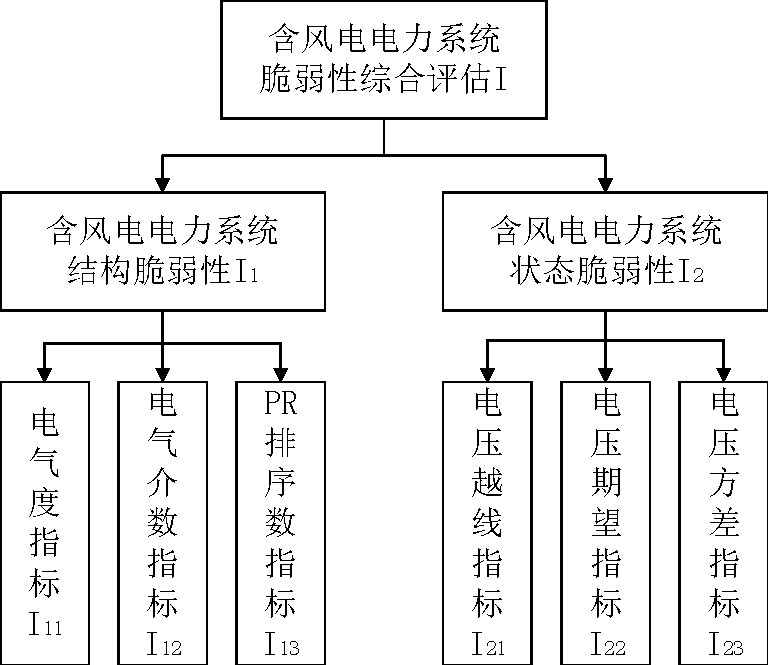
\includegraphics[height=6.8cm]{vulnerability_judgement.pdf}
  \caption{系统脆弱性综合评估指标集}
  \label{fig:vulnerability_judgement}
\end{figure}

\section{脆弱性量化评估二级指标融合}
\label{sec:processIndex}
由上述分析可知,系统的各个脆弱性评价指标分别从结构和状态的角度代表了系统脆弱性的不同属性,反应的是系统脆弱性现象的不同特征,每个指标的数量级都是不同的。因此,需要将这五个指标进行归一化处理,将数据统一映射到~[0,~1]~区间上,消除数量级的差异,从而将五个指标进行加权处理得到系统的综合脆弱性量化评估结果。

\subsection{脆弱性量化评估二级指标归一化}
\label{sec:nomalzMethod}
不同的数据格式及应用模型要求对数据采用不同的归一化方法,从而对特定的应用模型得到良好的数据分析效果。数据归一化的方法多种多样,常用的数据归一化方法见表~\ref{tab:chap4:normalize}。

其中针对评判指标的数据归一化方法主要采用离差标准化法及~z-score~标准化法。在分类、聚类等算法中,经常需要使用表征距离的数据来度量相似性,在主成分分析法~PCA~的计算过程中,需要对大量的数据进行降维,从而来去除数据中的噪声,挖掘数据中的模式。在这类问题中,z-score~数据归一化方式使得经过处理后的数据符合标准的正态分布特性,可以提升分类、聚类、主成分分析等算法模型的收敛速度及模型精度。但对于不涉及到距离度量计算、协方差计算且原始数据不符合高斯分布的时候,使用~z-score~数据归一化方法改变了原数据的分布特性,归一化处理后使得原有数据丢失了相应的信息。

\begin{table}[H]
\centering
\caption{常用的数据归一化方法 }\label{tab:chap4:normalize}
\begin{tabular}{C{3.8cm}C{2.9cm}C{2.7cm}C{3cm}}
\toprule
\textbf{方法} & \textbf{适用情况} & \textbf{特点} & \textbf{公式表示}\\
      \midrule
      %\tabincell{c}{}
        \tabincell{c}{离差标准化\\(Min-max Normalization)}
         & 适用于最大最小值明确不变的数据      & 不改变数据的原始分布      & $x^{\ast}=\FS{x-x_{min}}{x_{max}-x_{min}}$   \\

       z-score~标准化       & 适用于最大值最小值未知的情况,且数据接近正态分布
                                        & 改变数据的原始分布,对离群点规范化效果好            & $x^{\ast}=\FS{x-\mu}{\sigma}$       \\

      Logistic~标准化       & 适用于对长尾分布的数据作分段操作
                                        & 改变数据的分布情况             & $x^{\ast}=\FS{\ln x}{\ln n_{max}}$       \\

      \tabincell{c}{小数定标标准化\\(Decimal scaling)}    & 适用于数据初期探索,不消除数据属性间权重差异
                                       & 不改变数据分布                      & $x^{\ast}=\FS{x}{10j}$       \\

      排序归一化             & 适用于对数据的具体值并不关心,更关心相对排序的数据
                                       & 原始数据变为直线分布            & $x^{\ast}=\FS{x_{rank}}{num_{total}}$       \\

      分段归一化             & 适用于数据分布有明显分段特征的情况
                                       & 不改变分段数据的分布            & 根据不同数据段,采用不用方法       \\
\bottomrule
\end{tabular}
\end{table}

若明确知道数据的上限值和下限值,可以采用离差标准化的数据归一化方式进行数据处理。即不改变原有数据的分布规律,又将原始数据映射到~[0,~1]~数值区间内,消除了数据之间数量级的差异,解决了因量纲及数量级造成的可比性问题。又由于对原始数据的分布规律没有要求,且经过归一化处理后的数据可以进行相互比较与加权组合,使得离差标准化法成为建立综合评价体系时常用的归一化方式。

根据系统脆弱性综合评价指标及各指标的语义分析可知,系统结构脆弱性指标与系统状态脆弱性指标之间相互独立。由前文的分析知道系统的结构脆弱性反映了拓扑本身的性质,结构脆弱性的三个指标~$I_{11}$~、~$I_{12}$~与~$I_{13}$~都代表了节点在拓扑中的重要程度,即采用不同的建模方式均反映了节点在拓扑中的重要程度排位。其中,排位顺序是每个节点自身的属性,故三个脆弱性指标的归一化可以采用排序归一化,用顺序表明节点的相对重要性。

状态脆弱性指标通过仿真实验模拟了系统的性能的变化,所以状态指标属于评判性指标。由于脆弱性量化评价指标在数据分布上不符合标准正态分布特性,且归一化的主要目的是消除指标之间数量级的差异,并不涉及到距离度量计算和协方差计算。因此,本文在状态脆弱性指标的归一化中选择离差标准化方法。

离差标准化的指标归一化方法首先需要确定各指标的上限值和下限值,故首先要对系统的状态脆弱性指标的上限值和下限值进行分析确定。状态脆弱性指标$I_{21}$表示的是外界环境变化时,电压偏差状态无法使某些负荷正常运行的概率。所以该指标的上限值为$1$,下限值为$0$。状态脆弱性指标$I_{22}$表示的是环境发生变化时,电压偏差状态变化的期望,由于电压偏差$R$的本质是误差,故大小在$0-1$之间,所以其期望也在$ 0-1$之间。状态脆弱性指标$I_{23}$表示的是环境变化时,电压偏差状态变化的方差,所以该指标的变化范围也是$0-1$,因此该指标的上限值为$1$,下限值为$0$。

因此,经过归一化后的系统结构脆弱性指标向量为$I_{1}$和系统状态脆弱性指标向量为$I_{2}$。
\begin{equation}
\label{equ:chap4:Index5}
I_{1}=\left[~I_{11}^{\ast}~~~I_{12}^{\ast}~~~I_{13}^{\ast}~\right]
\end{equation}
\begin{equation}
\label{equ:chap4:Index6}
I_{2}=\left[~I_{21}^{\ast}~~~I_{22}^{\ast}~~~I_{23}^{\ast}~\right]
\end{equation}

\subsection{基于层次分析法的权重分配}
\label{sec:nomalz}
系统的脆弱性量化评估体系指的是在系统的工作环境大幅度变化或者意外发生的情况下,通过分别研究系统的拓扑和状态的变化选取特定的脆弱性评判指标来建立的。由于二级指标所显示出的系统性能的变化趋势对于系统脆弱性评判的重要程度具有较大的主观因素,因此系统脆弱性指标集的二级指标量化评估体系是一个基于主观评价的定权重综合评价体系。本文采用$AHP$(层次分析法)的相关理论,使用量化处理主观评价权重的方式对系统脆弱性评估指标进行权值分配。

判断各自二级指标之间的权重时,需要构建判断矩阵,将指标元素进行两两比较,根据主观定性的评价来度量准则~x~相比于准则~y~的重要程度。采用重要性量化标度~1-9~及其倒数对指标间的相对重要程度进行量化分析。若~x~相对于~y~的标度值大于~1,则表明~x~比~y~重要;若~x~相对于~y~的标度值小于~1,则表明~y~比~x~重要;当且仅当标度值为~1~时,表明~x~与~y~有相同的重要性。通过两两比较的方式,将二级指标之间相对重要性量化为~1-9~及其倒数,以此作为矩阵元素形成准则层的判断矩阵:
\begin{equation}\label{equ:chap4:Index8}
    A=\left(a_{ij}\right)_{m\times m}
\end{equation}

式中,A~~~为层次分析法某一层的判断矩阵;

\hspace{1.3cm}$a_{ij}$~为因素~i~针对于因素~j~的重要程度标度;

\hspace{1.3cm}m~~为该准则层元素的个数;

判断矩阵~1-9~重要性量化标度定义如表~\ref{tab:chap4:AHP_index}~所示

\begin{table}[H]
   \centering
  \renewcommand\arraystretch{1.3}
   \caption{判断矩阵~1-9~重要性量化标度}
   \label{tab:chap4:AHP_index}
     \begin{tabular}{|C{5cm}|C{8cm}|}
\hline
             重要性量化标度               &含义               \\
\hline
             1                                         &表示两个因素相比,前者与后者同等重要   \\
\hline
             3                                         &表示两个因素相比,前者比后者稍显重要  \\
\hline
             5                                         &表示两个因素相比,前者比后者明显重要   \\
\hline
             7                                         &表示两个因素相比,前者比后者强烈重要   \\
\hline
             2,~4,~6,~8                                &表示两个对象相比,前者比后者的重要程度介于上述相邻判断标度之间   \\
\hline
             倒数                                   &若因素~i~相对于因素~j~的重要性为~$a_{ij}$,则因素~j~相对于因素~i~的重要性
                                                           为~$a_{ji}=1\left. \right/a_{ij}$\\
\hline
\end{tabular}
\end{table}

为了保证基于层次分析法的判断意见合理准确,需要检验初始判断矩阵的一致性。根据矩阵论的相关知识,判断矩阵对应于最大特征值~$\lambda_{max}$~的特征向量经过归一化处理,即为同一层相应元素对应于上一层元素相对重要性的权值排序。由于满足式~\ref{equ:chap4:Index9}~的正互反矩阵被称为一致矩阵。根据定理可知,当且仅当~n~阶判断矩阵最大特征根~$\lambda_{max}=n$~时,判断矩阵为一致。当判断矩阵最大特征根~$\lambda_{max}>n$~时,判断矩阵非一致。 $\lambda_{max}$~比阶数~n~大的越多,判断矩阵的非一致性程度越大。
\begin{equation}\label{equ:chap4:Index9}
    a_{ij}a_{jk}=a_{ik},~~~~\forall i,j,k=1,2,\cdots n
\end{equation}

通常,判断矩阵的阶数越大,其具有完全一致性的难度越大,在层次分析法中虽然不要求判断矩阵完全一致,但要对判断矩阵的一致性满意程度进行度量。为了界定各个阶数判断矩阵的一致性满意度,定义一致性指标~CI~(Consistency Index)~和同阶评价随机一致性指标~RI~之比~CR~(Consistency Ratio)~为随机一致性比例\cite{Deng2012AHP},以此指标度量判断矩阵的一致性满意度。度量判断矩阵一致性的步骤如下~:

1)~计算一致性指标~CI~(Consistency Index)
\begin{equation}\label{equ:chap4:Index10}
    CI=\FS{\lambda_{max}-n}{n-1}
\end{equation}

式中,$\lambda_{max}$~为判断矩阵的最大特征值

\hspace{1.3cm}$n$~~为判断矩阵的阶数

2)~查询评价随机一致性指标~RI,如表~\ref{tab:chap4:consistency}~所示
\begin{table}[htb]
   \centering
 %  \renewcommand\arraystretch{1.5}
   \caption{平均随机一致性指标}
   \label{tab:chap4:consistency}

     \begin{tabular}{p{0.54cm}<{\centering}p{0.54cm}<{\centering}p{0.54cm}<{\centering}p{0.54cm}<{\centering}p{0.54cm}<{\centering}p{0.54cm}<{\centering}p{0.54cm}<{\centering}p{0.54cm}<{\centering}p{0.54cm}<{\centering}p{0.54cm}<{\centering}p{0.54cm}<{\centering}p{0.54cm}<{\centering}p{0.54cm}<{\centering}p{0.54cm}<{\centering}p{0.54cm}<{\centering}}
\toprule
n     & 1  &2  &3  &4  &5  &6   &7  &8   &9  &10   &11  &12    &13  &14    \\
\midrule
RI   &0.00  &0.00  &0.52  &0.89  &1.12 &1.24  &1.36  &1.41  &1.46  &1.49   &1.52  &1.54   &1.56  &1.58 \\
\bottomrule
\end{tabular}
\end{table}

3)~计算一致性比例~CR~(Consistency Ratio)
\begin{equation}\label{equ:chap4:Index11}
    CR=\FS{CI}{RI}
\end{equation}

4)~度量判断矩阵的一致性

根据一致性比例~CR~的计算结果,判断矩阵的一致性检测规则如下。

$CR<0.1$~:~说明判断矩阵具有良好的一致性,判断合理;

$CR=0.1$~:~说明判断矩阵具有较好的一致性,判断较为合理;

$CR>0.1$~:~说明判断矩阵不符合一致性原则,需要重新调整,直至满足一致性条件为止。

(4)~权重向量的计算

具有一致性的判断矩阵的最大特征根~$\lambda_{max}$~对应的特征向量经过归一化处理后,可以得到这一层元素对应于上一层元素相对重要性的权重向量。层次分析法中计算权重向量的方法主要有几何平均法~(\ref{equ:chap4:Index12})、算术平均法~(\ref{equ:chap4:Index13})~和特征向量法~(\ref{equ:chap4:Index14})~等。基于以上几种方法可以通过计算得到比较相近的权重向量,在实际应用过程中可根据需求选取相应合适的权重向量计算方式,得到科学有效的决策结果。
\begin{equation}\label{equ:chap4:Index12}
    W_i=\FS{\left(\prod\limits_{j=1}^{n}a_{ij}\right)^{\frac{1}{n}}}{\sum\limits_{i=1}^{n}\left(\prod\limits_{j=1}^{n}a_{ij}\right)^{\frac{1}{n}}},~~~~i=1,2,\cdots,n
\end{equation}
\begin{equation}\label{equ:chap4:Index13}
    W_i=\FS{1}{n}\sum_{j=1}^{n}\FS{a_{ij}}{\sum_{k=1}^{n}a_{kj}},~~~~i=1,2,\cdots,n
\end{equation}
\begin{equation}\label{equ:chap4:Index14}
    AW=\lambda_{max}W
\end{equation}

\subsection{脆弱性量化评估二级指标融合}
\label{sec:2ndIndexMerge}
本文所研究的含风电电力系统脆弱性问题,通过分析系统结构和系统状态来描述系统运行中潜在的缺陷,建立系统脆弱性量化评估模型。分别针对系统结构脆弱性和状态脆弱性的二级指标,采用层次分析法相关理论分配权重。对各自的二级评价指标进行两两比较,依据准则层元素间重要程度~1-9~标度可以得到如表~\ref{tab:chap4:importance1}~所示的结构脆弱性评价指标的重要性度量和如表~\ref{tab:chap4:importance2}~所示的状态脆弱性评价指标的重要性度量。

\begin{table}[htbp]
\centering
 \caption{系统结构脆弱性评价指标重要性度量}
  \label{tab:chap4:importance1}
\begin{tabular}{|C{2.5cm}|C{2.5cm}|C{2.5cm}|C{2.5cm}|}
\hline
             {名称}  &指标一       &指标二     &指标三\\
\hline
指标一 & 1 & 1/2 & 1\\
\hline
指标二 & 2 & 1 & 1\\
\hline
指标三 & 1 & 1 & 1\\
\hline
\end{tabular}
\end{table}

\begin{table}[htbp]
\centering
 \caption{系统状态脆弱性评价指标重要性度量}
  \label{tab:chap4:importance2}
\begin{tabular}{|C{2.5cm}|C{2.5cm}|C{2.5cm}|C{2.5cm}|}
\hline
             {名称}  &指标一       &指标二     &指标三\\
\hline
指标一 & 1 & 2 & 3\\
\hline
指标二 & 1/2 & 1 & 2\\
\hline
指标三 & 1/3 & 1/2 & 1\\
\hline
\end{tabular}
\end{table}

因此,可以得到系统结构脆弱性评价指标重要性度量初始判断矩阵~$A_1$~和系统状态脆弱性评价指标重要性度量初始判断矩阵~$A_2$~,利用~$MATLAB$~求解初始判断矩阵对应的特征根及特征向量,采用算数平均法对权重向量进行归一化,分别得出结构脆弱性量化评价指标的初始权重分配向量~$W(1)$~和状态脆弱性量化评价指标的初始权重分配向量~$W(2)$~分别为:
\begin{equation}\label{equ:chap4:Index15}
    W(1)=\left[~W_1~~W_2~~W_3~\right]=\left[~0.2599~~0.4126~~0.3275~\right]
\end{equation}
\begin{equation}\label{equ:chap4:Index16}
    W(2)=\left[~W_1~~W_2~~W_3~\right]=\left[~0.5396~~0.2970~~0.1634~\right]
\end{equation}

其对应的一致性比例分别为:

\begin{equation}\label{equ:chap4:Index17}
    CR_1=\FS{\lambda_{max}-n}{RI(n-1)}=\FS{3.0092-3}{0.58}=0.0462
    \end{equation}
\begin{equation}\label{equ:chap4:Index18}
    CR_2=\FS{\lambda_{max}-n}{RI(n-1)}=\FS{3.0536-3}{0.58}=0.0079
\end{equation}

由上式可知,结构脆弱性指标和状态脆弱性指标的一致性比例均满足~$CR<0.1$~的一致性检验标准,说明初始判断矩阵具有良好的一致性,判断合理。故初始脆弱性量化评价指标的权重分配向量~W~即为所求,各脆弱性评价指标的权重分配如图~\ref{fig:weightPie}~所示。由图可知,对系统结构脆弱性而言,指标二和指标三的影响最大。而对于系统状态脆弱性而言,指标一的影响最大。
\begin{figure}[H] % use float package if you want it here
  \centering
  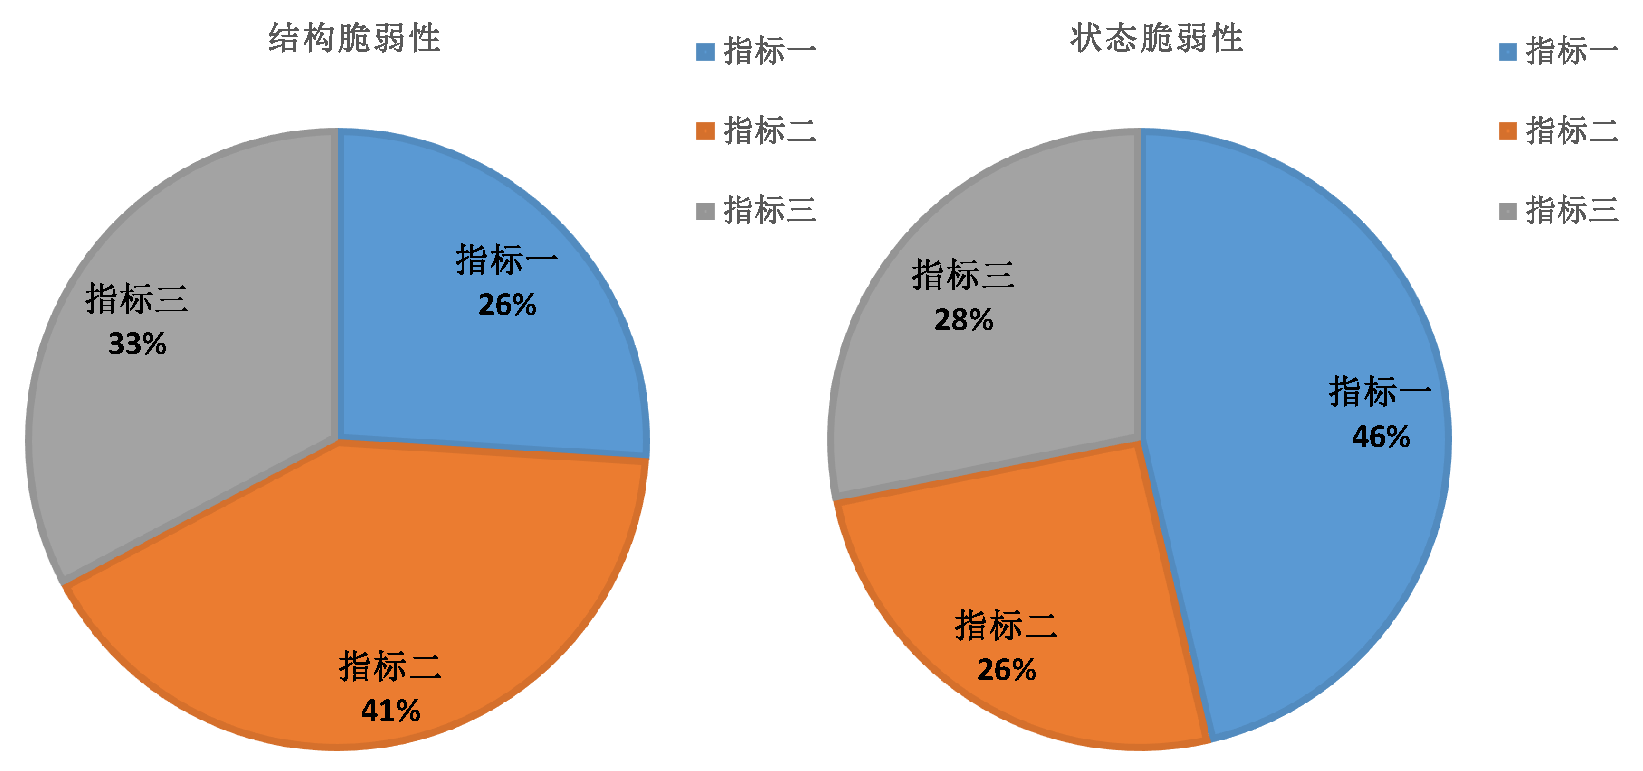
\includegraphics[height=6.9cm]{weightPie.pdf}
  \caption{系统脆弱性指标的权重分配图}
  \label{fig:weightPie}
\end{figure}

因此,分别对结构脆弱性的二级指标和状态脆弱性的二级指标进行融合如下:
\begin{equation}\label{equ:chap4:Index19}
\begin{split}
    V_1&=I_1\cdot W(1)^T\\
      &=\left[~I_{11}^{\ast}~~~I_{12}^{\ast}~~~I_{13}^{\ast}~\right]\cdot \left[~W_1~~W_2~~W_3~\right]^T,~~V_1\in \left[0,1\right]
\end{split}
\end{equation}
\begin{equation}\label{equ:chap4:Index20}
\begin{split}
    V_2&=I_2\cdot W(2)^T\\
      &=\left[~I_{21}^{\ast}~~~I_{22}^{\ast}~~~I_{23}^{\ast}~\right]\cdot \left[~W_1~~W_2~~W_3~\right]^T,~~V_2\in \left[0,1\right]
\end{split}
\end{equation}

\section{脆弱性量化评估一级指标融合}
\label{sec:quanIndex}
经过上述的研究分析可得到量化归一后的系统结构脆弱性指标~$V_1$~和系统状态脆弱性指标~$V_2$~,如何将这两个一级指标进行融合是本节研究的主要内容。考虑到这两个一级指标分别从不同的角度表征了系统的脆弱性,于是本文在研究$D-S$证据理论的基础上,进一步研究如何使用该方法来将脆弱性量化评估一级指标融合。

\subsection{$D-S$证据理论}
\label{sec:DStheory}
~$D-S$~证据理论是由$Dempster$提出的最早用于解决统计问题的方法,后来经$Shafer$推广发展称为一个更具普遍意义的用于处理不确定性问题的理论。~$D-S$~证据理论原理是利用上、下限概率解决多值映射问题,其核心优点在于可以将不同数据源利用$Dempster$合成规则进行综合,进一步由“证据”和“组合”来处理不确定性问题。

由于证据理论所需的先验数据比概率推理中的更直观且易获得,而且$Dempster$合成规则可以综合不同数据源的数据,这使得该理论在信息融合、情报分析、多属性决策分析、案件分析、专家系统等多领域有着广泛的应用\cite{DS1,DS2,DS3}。然而,该理论也存在一定的局限性,比如要求证据之间必须独立,计算上存在指数爆炸等问题。

本文的脆弱性量化评估一级指标融合问题中,由于一级指标分别从不同的角度进行脆弱性的评估,所以满足证据独立的特点。而且由于指标只有两个,并不存在计算上的指数爆炸的问题,因此可以使用该理论。~$D-S$~证据理论的基础包括以下三点:

$(1)$识别框架

识别框架指的是互不相容的事件(命题)的完备样本集合$\Theta$,表示为
\begin{equation}\label{equ:chap4:Index21}
\Theta={\theta_1,\theta_2,\cdots,\theta_n}
\end{equation}

$(2)$基本信任分配函数($BPA$)

设$\Theta$为识别框架,$\emptyset$为空集,若函数$m:2^{\Theta}\to[0,1]$($2^{\Theta}$为$\emptyset$的幂集)满足条件
\begin{equation}\label{equ:chap4:Index22}
\left\{\begin{array}{l}
        m(\emptyset)=0\\
        \sum_{A\subset\Theta}m(A)=1\\
\end{array}\right.
\end{equation}
则称$m$为框架$\Theta$上的基本信任分配函数($mass$函数),$\forall A\subset\Theta$,$m(A)$为$A$的基本信任分配值,其中,使得$m(A)>0$的$A$称为焦元。

$(3)$证据理论合成规则

2个证据合成:

假设$m_1$和$m_2$分别是同一识别框架$\Theta$上的2个基本信任分配函数,$m_1$、$m_2$的焦元分别为$A_i$和$B_j$,设$K=\sum_{A_i\cap B_j}m_1(A_i)m_2(B_j)<1$,若映射$m:2^{\Theta}\to[0,1]$,则合成规则为:
\begin{equation}\label{equ:chap4:Index23}
m(A)= \begin{cases}
        0 & A=\Theta\\
        \displaystyle\frac{\sum_{A_i\cap B_j}m_1(A_i)m_2(B_j)}{1-K} & A\neq \Theta\\
      \end{cases}
\end{equation}

多个证据合成:

假设$m_1$,$m_2$,$\cdots$,$m_r$分别是同一识别框架$\Theta$上的2个基本信任分配函数,对应的焦元分别为$A_i(i=1,2,\cdots,r)$,设$K=\sum_{A_1\cap \cdots \cap A_r = \emptyset}m_1(A_1)m_2(A_1)\cdots m_r(A_r)<1$,若映射$m:2^{\Theta}\to[0,1]$,则$r$条证据的合成规则为:
\begin{equation}\label{equ:chap4:Index24}
m(A)= \begin{cases}
        0 & A=\Theta\\
        \displaystyle\frac{\sum_{A_1\cap A_2\cap \cdots \cap A_r=A}m_1(A_1)m_2(A_2)\cdots m_r(A_r)}{1-K} & A\neq \Theta\\
      \end{cases}
\end{equation}

基于~$D-S$~理论的不确定性推理步骤如图\ref{fig:DSliucheng}。由图可知,该理论的推理首先要确定概率分配函数($BPA$),进而将证据数据知识的不确定性用$BPA$函数来表示。然后确定组合证据不确定性的算法,进行$Dempster$证据合成,从而得到最终的推理结果。
\begin{figure}[H] % use float package if you want it here
  \centering
  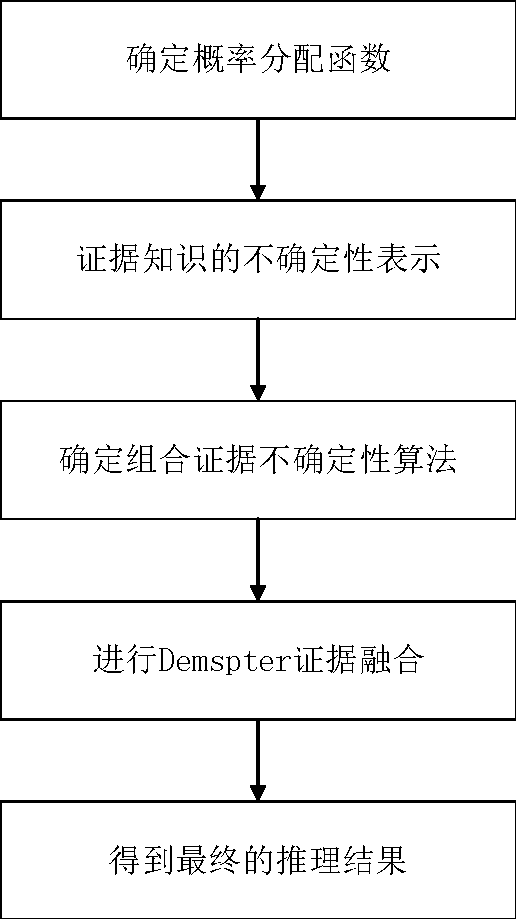
\includegraphics[height=8.3cm]{DSliucheng.pdf}
  \caption{基于~$D-S$~理论的不确定性推理步骤图}
  \label{fig:DSliucheng}
\end{figure}
\subsection{脆弱性量化评估一级指标融合}
\label{sec:DSdistri}
本文的系统脆弱性一级指标主要指的是结构脆弱性指标$V_1$和状态脆弱性指标$V_2$,由于这两个指标分别从不同方向描述受到威胁后系统受影响的程度,因此两个指标可以视为独立的两条证据。鉴于$D-S$证据理论最大的特点是基于不确定的信息描述来估计不确定性的区间,所以脆弱性量化评估一级指标融合的问题可以用$D-S$证据理论的方法进行解决。

由前文可知,系统结构脆弱性指标$V_1$和系统状态脆弱性指标$V_2$采用层次分析法进行量化归一后,两个指标的上限阈值都是0,代表系统是反脆弱的,系统绝对好。指标的下限阈值都是1,代表系统是极脆弱的,系统绝对差。因此,两个指标的证据$P_1$、$P_2$可以表示为:
\begin{equation}\label{equ:chap4:Index26}
P_1=V_1\times 100\%
\end{equation}
\begin{equation}\label{equ:chap4:Index27}
P_2=V_2\times 100\%
\end{equation}

两个证据的取值均为$0-1$,设其相应的识别框架定义为:
\begin{equation}\label{equ:chap4:Index28}
\Theta = \{antivulnerable,vulnerable\}
\end{equation}

则可定义如下的$BPA$函数:
\begin{equation}\label{equ:chap4:Index29}
m_1(\{antivulnerable\},\{vulnerable\})=(1-P_1,P_1)
\end{equation}
\begin{equation}\label{equ:chap4:Index30}
m_2(\{antivulnerable\},\{vulnerable\})=(1-P_2,P_2)
\end{equation}

在获得了两个指标的$BPA$之后,就可以用$Dempster$合成规则融合2个$BPA$值,从而得到系统的脆弱性描述。根据合成规则的公式\ref{equ:chap4:Index23},定义脆弱性指数$VI$如下:
\begin{equation}\label{equ:chap4:Index31}
\begin{split}
   VI& =\{vulnerable\} \\
     & =\displaystyle\frac{\sum_{X\cap Y=\{vulnerable\}}m_1(X)m_2(Y)}{\sum_{X\cap Y\neq {\emptyset}}m_1(X)m_2(Y)} \\
     & =\frac{P_1 \times P_2}{P_1 \times P_2+(1-P_1) \times (1-P_2)}
\end{split}
\end{equation}

可以看出,$VI$值代表了系统的脆弱性指数,它结合了系统结构脆弱性指标与系统状态脆弱性指标这两个一级指标。而一级指标由各自的二级指标融合得到,因此$VI$值综合评估了含风电电力系统的脆弱性,具有普适意义。$VI$值越大,代表着系统越脆弱,系统越差。反之,系统具有的脆弱性越小,代表系统越好。

\section{系统脆弱性量化评价体系描述}
\label{sec:systemQuan}
结合第三章含风电电力系统的脆弱性研究以及上述系统脆弱性量化评估指标及系统脆弱性量化评估指标融合的研究可知,建立控制系统脆弱性量化评价体系的数学模型主要有以下两部分工作。

首先,根据含风电电力系统的组成和特性,建立了系统模型。然后,在研究了含风电电力系统的脆弱性本质和数学描述的基础上,分别从结构脆弱性和状态脆弱性两方面进行研究。对于系统结构脆弱性,分别基于复杂网络和$PageRank$进行建模。对于系统状态脆弱性,则采用蒙特卡洛的概率潮流进行建模。

其次,对于得到的结构脆弱性模型,根据系统结构脆弱性的定义,分别计算出表征拓扑连接强度的电气度指标$I_{11}$、表征拓扑能量传输分布的电气介数指标$I_{12}$、表征拓扑重要性的$PR$排序数指标$I_{13}$。将这些指标归一化后得到系统结构脆弱性指标向量$I_{1}=\left[~I_{11}^{\ast}~~~I_{12}^{\ast}~~~I_{13}^{\ast}~\right]$。同理,根据系统状态脆弱性的定义,分别计算出表征环境变化导致系统具有脆弱性可能的电压越线率指标$I_{21}$、表征系统电压偏差状态变化均值的电压期望指标$I_{22}$、表征系统电压状态偏差状态变化剧烈程度的电压方差指标$I_{23}$。再将指标归一化后得到系统状态脆弱性指标向量$I_{2}=\left[~I_{21}^{\ast}~~~I_{22}^{\ast}~~~I_{23}^{\ast}~\right]$。采用层次分析法分别对各自的脆弱性量化指标进行权重分配,得到权重分配向量W(1)和W(2),进一步得到结构脆弱性指标$V_1=\left[~I_{11}^{\ast}~~~I_{12}^{\ast}~~~I_{13}^{\ast}~\right]\cdot \left[~W_1~~W_2~~W_3~\right]^T$和状态脆弱性指标$V_2=\left[~I_{21}^{\ast}~~~I_{22}^{\ast}~~~I_{23}^{\ast}~\right]\cdot \left[~W_1~~W_2~~W_3~\right]^T$。最后,采用$D-S$证据理论将结构脆弱性指标与状态脆弱性指标进行融合,得到系统综合脆弱性指标$VI$。至此,本文研究的含风电电力系统脆弱性量化评估体系数学模型建立完毕。

\section{本章小结}
\label{sec:sum4}
本章在系统脆弱性的研究基础上,根据脆弱性的定义与特征,针对结构脆弱性和状态脆弱性分别选取了3个能够反映脆弱性的指标,从而得到系统脆弱性综合评估指标集,其中对一级指标和二级指标进行了定义与区分。鉴于系统脆弱性问题的主观性,对系统脆弱性量化评估体系问题进行分析与研究。

针对脆弱性二级指标首先选择合适的方法进行归一化处理,然后采用层次分析法进行权重分配,得到结构脆弱性和状态脆弱性的一级指标。最后,在$D-S$证据理论的研究基础上,将结构脆弱性指标与状态脆弱性指标进行融合,得到了系统综合脆弱性指标,为后文的脆弱性量化分析提供理论基础。



